\makeatletter
\def\input@path{{../styles/}{../../styles/}{../../../styles/}{../}{../../}{../../../}}
\makeatother
\documentclass{ee102_notes}
% macros.tex - Course meta information
\renewcommand{\course}{EE 102}
\renewcommand{\coursetitle}{Signal Processing and Linear Systems}
\renewcommand{\instructor}{Ayush Pandey}
\renewcommand{\semester}{Fall}
\renewcommand{\year}{2025}
\renewcommand{\shorttitle}{Week 1: Introduction to Signals}
% Use \renewcommand to avoid 'already defined' errors

% The following packages can be found on http:\\www.ctan.org
% \usepackage{graphics} % for pdf, bitmapped graphics files
%\usepackage{epsfig} % for postscript graphics files
%\usepackage{mathptmx} % assumes new font selection scheme installed
%\usepackage{times} % assumes new font selection scheme installed
\usepackage{amsmath} % assumes amsmath package installed
\usepackage{amssymb,mathtools}  % assumes amsmath package installed
\usepackage{xcolor}
\usepackage{pgfplots,subcaption}
\usepackage[hidelinks]{hyperref}
\usepackage{verbatim}
\usepackage{graphicx}
\usepackage{listings}

% -------- listings (Python) ----------
\lstdefinestyle{py}{
  language=Python,
  basicstyle=\ttfamily\small,
  keywordstyle=\color{blue!60!black}\bfseries,
  commentstyle=\color{green!40!black},
  stringstyle=\color{orange!60!black},
  showstringspaces=false,
  columns=fullflexible,
  frame=single,
  framerule=0.3pt,
  numbers=left,
  numberstyle=\tiny,
  xleftmargin=1em,
  tabsize=2,
  breaklines=true,
}
\usepackage[american]{circuitikz}
\usepackage{tikz}
\usepackage{caption}    
\usepackage{lscape}
\usepackage{soul}
\usepackage{tikz}
\usetikzlibrary{calc,angles,quotes,arrows.meta}

\usepackage{hyperref}
\hypersetup{
    colorlinks=true,
    linkcolor=blue,
    filecolor=magenta,      
    urlcolor=blue,
    pdftitle={week1_notes},
    pdfpagemode=FullScreen,
}
%\usepackage{float} 

%\usepackage[demo]{graphicx}
\pgfplotsset{compat=1.18}
% \usepgfplotslibrary{fillbetween}

\newsavebox{\measurebox}

\let\proof\relax\let\endproof\relax


\newcommand{\norm}[1]{\left\lVert#1\right\rVert}
\def\abs#1{\left\lvert#1\right\rvert}
\let\proof\relax
\let\endproof\relax
\usepackage{amsthm}
\usepackage{accents}
\usepackage{relsize}
\newcommand{\ubar}[1]{\underaccent{\bar}{#1}}
\newtheorem{theorem}{Theorem}
\newtheorem{corollary}{Corollary}[theorem]
\newtheorem{lemma}{Lemma}
\newtheorem{proposition}{Proposition}
\newtheorem{statement}{Statement}

\theoremstyle{definition}
\newtheorem{definition}{Definition}
 
\theoremstyle{remark}
\newtheorem*{remark}{Remark}
\theoremstyle{remark}
\newtheorem*{claim}{Claim}
\setlength{\parindent}{0cm}
\newenvironment{nalign}{
    \begin{equation}
    \begin{aligned}
}{
    \end{aligned}
    \end{equation}
    \ignorespacesafterend
}

\renewcommand{\releasedate}{October 20, 2025}

\newcommand{\Eblank}{\rule{3cm}{0.4pt}}
\newcommand{\Rankblank}{\rule{3cm}{0.4pt}}

\begin{document}
\section*{EE 102 Week 8, Lecture 1 (Fall 2025)}
\subsection*{Instructor: \instructor}
\subsection*{Date: \releasedate}

\section{Goals}
The overall goal in EE 102 is to break down signals into its constituent fundamental components that can be easily analyzed. So far, we have achieved this in two ways: we have broken down any arbitrary signal into impulse signals, and we have broken down periodic signals into sinusoids. What's left? Signals that are not periodic. So, our goal is \dots 

By the end of this lecture, you should be able to break down aperiodic signals into their constituent frequency components using Fourier Transform.
% ---------- Pop-Quiz 1 ----------
\section{Review: Decomposition of signals}
In this section, we review how to decompose signals into simpler components. We have already seen two ways to do this: using impulses and using sinusoids. We will work through one example of each. 
\subsection{Breaking down signals using impulses}
Choose a signal $x(t)$ --- scribble something! Break it down so that it can be constructed using only impulses $\delta(t)$ with appropriate scales and shifts.

\medskip
\textbf{(a) Show it visually: } On the left, sketch $x(t)$. On the right, place weighted impulses at sample locations corresponding to the value of $x(t)$ at those locations. Note that integer times are shown here, but you may choose any sampling interval (can be floating point because this is a continuous-time signal).

\begin{center}
\begin{minipage}{0.5\linewidth}
\begin{tikzpicture}[x=0.7cm,y=0.9cm]
  \draw[->] (-4.6,0) -- (4.6,0) node[below] {$t$};
  \draw[->] (0,-2.2) -- (0,2.6) node[left] {$x(t)$};
  \foreach \xx in {-4,-3,-2,-1,1,2,3,4}{\fill[black!25] (\xx,0) circle(0.03);}
  \foreach \yy in {-2,-1,1,2}{\fill[black!25] (0,\yy) circle(0.03);}
  \node[align=center] at (0,3.2) {\small Sketch $x(t)$ here};
\end{tikzpicture}
\end{minipage}\hfill
\begin{minipage}{0.5\linewidth}
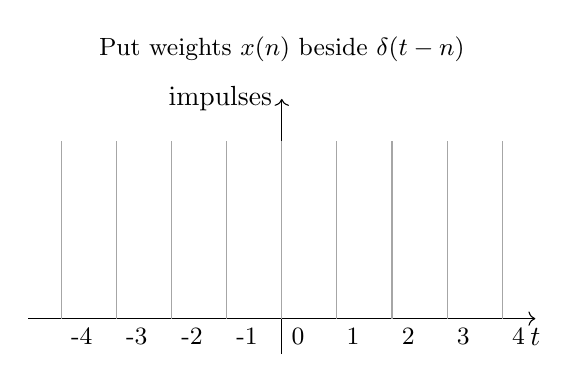
\begin{tikzpicture}[x=0.7cm,y=0.9cm]
  \draw[->] (-4.6,0) -- (4.6,0) node[below] {$t$};
  \draw[->] (0,-0.5) -- (0,3.1) node[left] {impulses};
  \foreach \n in {-4,-3,-2,-1,0,1,2,3,4}{
     \draw[black!35] (\n,0) -- ++(0,2.5);
     \node[below right] at (\n,0) {\small \n};
  }
  \node[align=center] at (0,3.8) {\small Put weights $x(n)$ beside $\delta(t-n)$};
\end{tikzpicture}
\end{minipage}
\end{center}

\medskip
\textbf{(b) Do it mathematically:} Use the sifting property to write a formula for $x(t)$ using $\delta(\cdot)$.

\fbox{\begin{minipage}[t][3.0cm][t]{0.98\linewidth}
\vspace{0.2cm}
\textit{Write your mathematical expression here:}
\end{minipage}}

\textbf{Possible solution}
We sketch $x(t)$ as a continuous curve on the left, and place impulses at various locations, which is shown on the right. 
\begin{center}
\begin{minipage}{0.47\linewidth}
\begin{tikzpicture}[x=0.9cm,y=0.9cm]
  \draw[->] (-4.6,0) -- (4.6,0) node[below] {$t$};
  \draw[->] (0,-2.2) -- (0,2.6) node[left] {$x(t)$};
  \draw[very thick] (-4,0.2) .. controls (-2,1.6) and (-1.2,1.8) .. (0,0.3)
                     .. controls (0.7,-0.2) and (2,0.8) .. (3.3,1.6)
                     .. controls (3.7,1.9) and (4.2,1.2) .. (4.3,0.1);
\end{tikzpicture}
\end{minipage}\hfill
\begin{minipage}{0.47\linewidth}
\begin{tikzpicture}[x=0.9cm,y=0.9cm]
  \draw[->] (-4.6,0) -- (4.6,0) node[below] {$t$};
  \draw[->] (0,-0.5) -- (0,3.1);
  \foreach \n/\h in {-4/0.5,-3/1.1,-2/1.8,-1/2.4,0/0.7,1/0.3,2/1.4,3/2.2,4/1.0}{
     \draw[very thick] (\n,0) -- ++(0,\h);
     \fill (\n,\h) circle(0.05);
  }
\end{tikzpicture}
\end{minipage}
\end{center}

Mathematically, we have the sifting property of the impulse:
\[\,x(t)=\int_{-\infty}^{\infty} x(\tau)\,\delta(t-\tau)\,d\tau\,
\] 
which can be approximated using a sum over discrete time instants as
\[
\,x(t)\approx \sum_{n=-\infty}^{\infty} x(n)\,\delta(t-n)\, .
\]

\subsection{Breaking down periodic signals using sinusoids}
Draw an impulse train with period $T_0$. Then, sketch (approximately) how a finite sum of sinusoids could approximate this train over time. Finally, write the corresponding Fourier-series form and coefficients.

\fbox{\begin{minipage}[t][3.0cm][t]{0.98\linewidth}
\vspace{0.2cm}
\textit{Write $x(t)=\sum_{k=-\infty}^{\infty} a_k e^{jk\omega_0 t}$ and specify $a_k$. Optionally write the finite $N$-term partial sum you would draw.}
\end{minipage}}


Finally, consider a $50\%$ duty cycle symmetric square wave of amplitude $A$ and period $T_0=\dfrac{2\pi}{\omega_0}$. Sketch one period on an axes, draw the first few nonzero harmonic magnitudes, and write the Fourier series formula you would use to represent this signal.
% \textbf{(b)} On the right, draw the first few harmonic magnitudes (only nonzero ones).

\fbox{\begin{minipage}[t][3.2cm][t]{0.98\linewidth}
\vspace{0.2cm}
\textit{Write the FS synthesis and the coefficients for a $50\%$ duty square wave of amplitude $A$.}
\end{minipage}}

\paragraph{Why/how is that useful?}

After you have worked through the above examples, you are all set up to compute the output of any LTI system. To achieve that you would need the following additional information (one or the other): 
\begin{itemize}
    \item How does the system respond to an impulse input? (i.e., the impulse response of the system, $h(t)$)
    \item How does the system respond to sinusoidal inputs? (i.e., the frequency response of the system, $H(f)$)
\end{itemize}
Then, you can compute the output of the system for any arbitrary input signal $x(t)$ using either convolution or the Fourier synthesis equation (and LTI system properties!).

\section{Fourier Transform: Decomposition of aperiodic signals}

The \ul{\textbf{key idea}} in this lecture is that aperiodic signals are also periodic signals, but with the time period $T \to \infty$. That is, the aperiodic signal also repeats itself, but only after an infinite amount of time has passed! This essentially means that it never repeats itself (inifinite is not defined).

So, let's try to apply that idea with an example. Consider a square wave of magnitude $A$, centered around 0, with a period of $T$. For the period between $-T/2$ and $T/2$, the signal is defined as:
\[
x(t) = \begin{cases}
A, & -T_1 \le t \le T_1,\\
0, & \text{otherwise.}
\end{cases}
\]
We can find the Fourier series coefficients for this signal using the Fourier series analysis equation:
\[
a_k = \frac{1}{T} \int_{-T/2}^{T/2} x(t) e^{-jk\omega_0 t} dt,
\]
where $\omega_0 = \dfrac{2\pi}{T}$. Note that the limits of integration should be (ideally, according to the formula for $a_k$) over one period of the signal. However, since $x(t)$ is zero outside the interval $[-T_1, T_1]$, we can simplify the limits of integration to:
\[
a_k = \frac{1}{T} \int_{-T_1}^{T_1} A e^{-jk\omega_0 t} dt.
\]
Evaluating this integral, we get:
\begin{align*}
    a_k &= \frac{A}{T} \int_{-T_1}^{T_1} e^{-jk\omega_0 t} dt \\
    &= \frac{A}{T} \left[ \frac{e^{-jk\omega_0 t}}{-jk\omega_0} \right]_{-T_1}^{T_1} \\
    &= \frac{A}{T} \left( \frac{e^{-jk\omega_0 T_1} - e^{jk\omega_0 T_1}}{-jk\omega_0} \right) \\
    &= \frac{A}{T} \left( \frac{-2j \sin(k\omega_0 T_1)}{-jk\omega_0} \right) \\
    &= \frac{2A}{T} \cdot \frac{\sin(k\omega_0 T_1)}{k\omega_0}.
\end{align*}
For convenience, we define a new function called the \textbf{sinc function} as (pronounced ``sink''):
\[
\textrm{sinc}(x) = \frac{\sin(x)}{x}.
\]
We can now rewrite the Fourier series coefficients as:
\[
a_k = \frac{2A T_1}{T} \textrm{sinc}(k\omega_0 T_1).
\]
Now, since $T \to \infty$, let's re-write the left-hand side as 
\[
T a_k = 2AT_1 \textrm{sinc}(k\omega_0 T_1).
\]
Notice that as $T \to \infty$, the fundamental frequency $\omega_0 = \frac{2\pi}{T} \to 0$. The right hand side expression above is a function of frequency: $2A T_1 \textrm{sinc}(k\omega_0 T_1)$. Since $\omega_0 \to 0$, we make a very important observation. The function of frequency can be defined as a continuous function in the limit. You can see this with the following re-definition:
\[
\omega_0 := \Delta \omega 
\] 
and then $k \omega_0 = k \Delta \omega$, which in turn we define as $\omega := \omega_k := k \Delta \omega$.

Intuitively, if you think of the frequency as the X-axis, then the Fourier series coefficients can be thought of as samples of a continuous function in the limit as $T \to \infty$. This is the key idea behind the Fourier transform: it allows us to represent aperiodic signals as a continuous sum of sinusoids, each with a specific frequency and amplitude.

For the square wave example above, we then have
\[
T a_k = 2 A T_1 sinc(\omega T_1)
\]
which can be further interpreted as  
\[
2\pi a_k = \left[2A T_1 sinc(\omega T_1) \right] \Delta \omega.
\]
This frequency function is called the Fourier transform of the signal. What we have done is that we started from from a continuous-time (in time domain), which we have now \emph{transformed} into a function of frequency (in frequency domain).

\section{The Fourier Transform}
For a general aperiodic signal $x(t)$, the Fourier transform can be derived using the Fourier series synthesis and analysis equations:
\begin{align*}
    x(t) &= \sum_{k=-\infty}^{\infty} a_k e^{jk\omega_0 t}, \\
    a_k &= \frac{1}{T} \int_{-T/2}^{T/2} x(t) e^{-jk\omega_0 t} dt. \\
    \text{As } T \to \infty, \text{ we have:} \\
    \omega_0 &= \frac{2\pi}{T} \to 0.
    \text{Thus, we can write:} \\
    T a_k &= \int_{-\infty}^{\infty} x(t) e^{-j\omega t} dt,
\end{align*}
where we used the definition of frequency $\omega = k \omega_0$. Now, we can rewrite the synthesis equation as:
\begin{align*}
    x(t) &= \frac{1}{2\pi} \int_{-\infty}^{\infty} \left[ \int_{-\infty}^{\infty} x(\tau) e^{-j\omega \tau} d\tau \right] e^{j\omega t} d\omega.
\end{align*}
We define the above as the Fourier transform pair:
\[
X(\omega) = \int_{-\infty}^{\infty} x(t) e^{-j\omega t} dt,
\]
\[
x(t) = \frac{1}{2\pi} \int_{-\infty}^{\infty} X(\omega) e^{j\omega t} d\omega.
\]
This pair of equations allows us to transform a time-domain signal $x(t)$ into its frequency-domain representation $X(\omega)$ and vice versa! We will work on specific examples in the next class.

\section{Recommended reading and practice problems}
\begin{itemize}
    \item Solved example 3.5 in Oppenheim and Willsky, 2nd edition.
    \item Example 4.1 in Lathi.
\end{itemize}
\end{document}
